\documentclass{standalone}

\usepackage{lscape}
%Math typesetting packages
\usepackage{amsfonts, amssymb, amsmath, latexsym, amsthm,xparse}
\newcommand\simiid{\stackrel{iid}{\sim}}
\newcommand\simind{\stackrel{ind}{\sim}}
\NewDocumentCommand{\qfrac}{smm}{%
  \dfrac{\IfBooleanT{#1}{\vphantom{\big|}}#2}{\mathstrut #3}%
}

\usepackage{tikz}
\usetikzlibrary{calc,arrows,positioning,shapes,shapes.gates.logic.US,trees, intersections}

\begin{document}

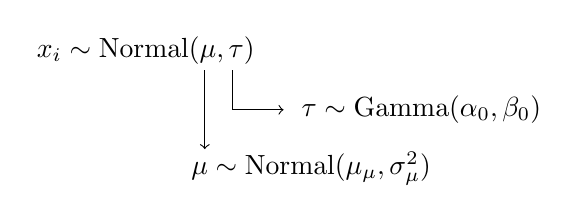
\begin{tikzpicture}
  \node at (0,0) {$x_i \sim \mathrm{Normal}(\mu, \tau)$} ;
  	\draw[->] (0.75,-0.25) to (0.75,-1.25);
  	\node at (2.1, -1.5) {$\mu\sim \mathrm{Normal}(\mu_{\mu},\sigma^2_{\mu})$};
  	\draw[->] (1.1, -0.25) |- (1.75, -0.75);
  	\node at (3.5, -0.75) {$\tau\sim \mathrm{Gamma}(\alpha_0, \beta_0)$};
\end{tikzpicture}

\end{document}